\documentclass{book}

\usepackage{graphicx}
\usepackage[italian]{babel}
%\usepackage{listings}
%\usepackage[export]{adjustbox}
\usepackage{hyperref}
\hypersetup{linktoc=all}


\begin{document}
    
\author{Giovanni Tosini}
\title{Sistemi Operativi \\
\large Secondo semestre}
\date{ }
\maketitle
\newpage
\tableofcontents
\newpage

\section{Monitor}

Si tratta di una struttura simile ai semafori, implementa di default la mutua esclusione. Simile a una classe di un linguaggio a oggetti, può contenere:
\begin{itemize}
    \item variabili(sono private)
    \item metodi(solo loro possono utilizzare le variabili definite all'interno del Monitor)
    \item costruttore
\end{itemize}

Quando un processo usa una entry del Monitor, gli altri non possono accedervi. Al suo interno posso dichiarare variabili di tipo CONDITION, non hanno valore, vengo usate esclusivamente con i metodi WAIT e SIGNAL.

\begin{verbatim}
    CONDITION x
    x.wait -> blocca il processo, non avvengono incrementi
              o decrementi come con i semafori
    x.signal -> se fatto quando non ci sono processi in
                attesa, non fa niente
\end{verbatim}

\begin{center}
    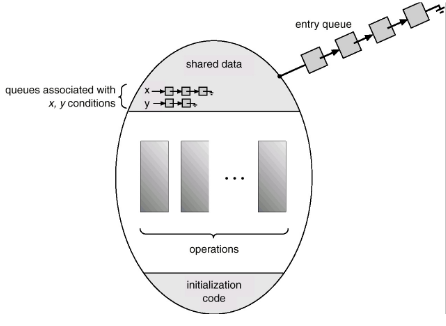
\includegraphics[width=0.5\textwidth]{ovetto.png}
\end{center}

Il comando SIGNAL può rompere la mutua esclusione, perché un eventuale processo fermo potrebbe ripartire e in quel caso entrambi sarebbe all'interno della sezione critica, per evitare ciò il processo che la chiama:
\begin{itemize}
    \item viene bloccato
    \item oppure SIGNAL deve essere l'ultima istruzione prima di uscire dal Monitor
\end{itemize}

Quale metodo usare? Dipende dal Monitor.

\subsection{Problematiche}

\begin{itemize}
    \item esistono pochi linguaggi che li implementano
    \item possono essere applicati solo quando ci sono processi che condividono la memoria(stessa macchina)
\end{itemize}

\section{Deadlock}

Causato quando un processo è in attesa di un evento causato a sua volta da un altro processo in attesa.
Ci sono quattro condizioni che possono causare un Deadlock:

\begin{itemize}
    \item mutua esclusione
    \item hold and wait: processo che detiene una risorsa ed è in attesa di una risorsa utilizzata da un altro
    \item no preemption: il processo deve rilasciare volontariamente la risorsa(non può essere ucciso)
    \item catena circolare: A attende B, che attende C, che attende A
\end{itemize}
In presenza di tutte e quattro esiste la possibilità che si verifichi.
Tecnica di prevenzione: basta che una delle quattro non venga rispettata e il Deadlock non può avvenire.

\paragraph{Modello astratto RAG (Resource Allocation Graph)}

\begin{center}
    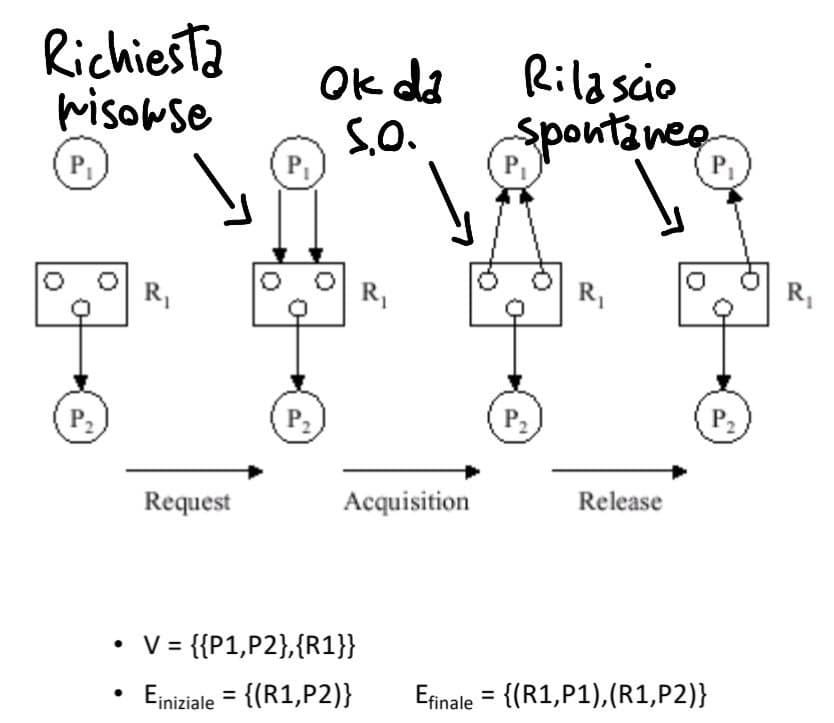
\includegraphics[width=0.5\textwidth]{rag.jpg}    
\end{center}
In generale, se abbiamo una sola istanza di ogni risorsa e siamo in presenza di un ciclo, il Deadlock è certo.
Con risorse con più istanze invece non è assicurato.

\subsection{Gestione Deadlock}

Prevenzione statica: evitare ovvero che si verifichino una della quattro condizioni sopra riportate,
se ci sono risorse disponibili non le assegno a prescindere.

\begin{itemize}
    \item mutua esclusione: non posso toglierla
    \item hold and wait: accumulo tutte le risorse tutte in una volta altrimenti non procedo
    questo porta a delle problematiche:
    \begin{itemize}
        \item basso uso delle risorse
        \item starvation
        \item occorre conoscere le risorse necessarie
    \end{itemize}
    \item no preemption: un processo che richiede una risorsa non disponibile
    sarà costretto a rilasciare tutte le altre risorse che stava tenendo
    \item ogni risorsa avrà una priorità crescente, il processo può richiederle esclusivamente in ordine crescente
\end{itemize}
Prevenzione dinamica, durante l'esecuzione si blocca un processo in base al RAG, occorre conoscere  a priori il caso peggiore 
in cui si causa un Deadlock e permette di sfruttare maggiormente le risorse per altri processi diversamente da quella statica.
Guardando il RAG, come un processo richiede una risorsa ipotizza di concederla e verifica se si presenta un ciclo,
in caso affermativo la richiesta verrà rifiutata, il processo rimarrà in attesa e il sistema resterà in 
un stato SAFE.

\vspace{3ex}
\begin{tabular}{|c|c|c|}
    \hline
    x & Richieste & Possedute \\
    \hline
    p0 & 10 & 5 \\
    \hline
    p1 & 4 & 2 \\
    \hline
    p2 & 9 & 2 \\
    \hline    
\end{tabular}

\vspace{3ex}p0 avrà bisogno di 10 istanze delle quali già ne possiede 5,12 sono quelle presenti, 9 in uso e 3 libere.
Stato SAFE o UNSAFE? Si va in ordine per processo:

\begin{itemize}
    \item p0 ne sta usando 5, ne occorrono altre 5, con le 3 libere non può essere soddisfatto, di conseguenza rimarrà in attesa
    \item p1 ne chiede 4, ne ha già 2, 3 sono libere, di conseguenza se andasse prima lui ne avremmo 5 libere dopo
\end{itemize}
Quindi saremmo in uno stato SAFE.\\
N.B.: lo scheduler in tutto ciò non ha rilevanza, lui si limita scegliere quali processi mettere nella CPU.

Lo svantaggio della
previsione dinamica è l'uso delle risorse minore, perché ci possono esserne alcune che non vengono sfruttate.

\vspace{3ex}1) L'algoritmo RAG funziona solo con risorse che possiedono un'unica istanza, funzionamento:

\begin{itemize}
    \item aggiungo al RAG l'arco di reclamo, ovvero in futuro quel processo richiederà l'uso di quella risorsa molto probabilmente
    \item il S.O. permetterà al processo di usare la risorsa solo se ipotizzando che venga fatto, non si verifichi un ciclo
\end{itemize}

\begin{center}
    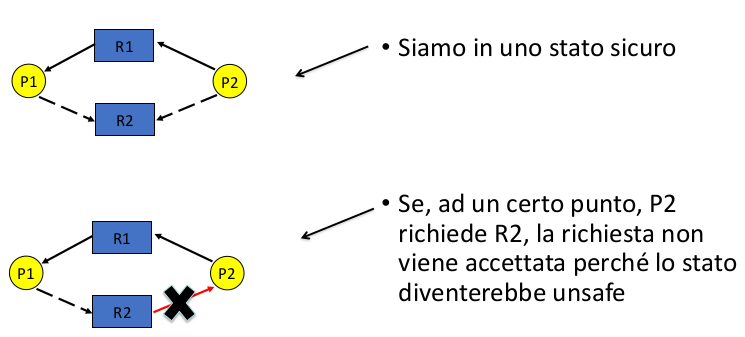
\includegraphics[width=0.8\textwidth]{rag_reclamo.png}
\end{center}
La freccia tratteggiata indica l'arco di reclamo.

2) L'algoritmo del banchiere è meno efficiente dell'algorimo RAG, ma
funziona con qualsiasi numero di istanze delle risorse. Si divide in due parti, una che simula la cessione dell'istanza della risorsa
e una che ne verifica l'effetto.

\begin{center}
    \includegraphics*[width=1\textwidth]{banchiere3.png}
\end{center}

\begin{center}
    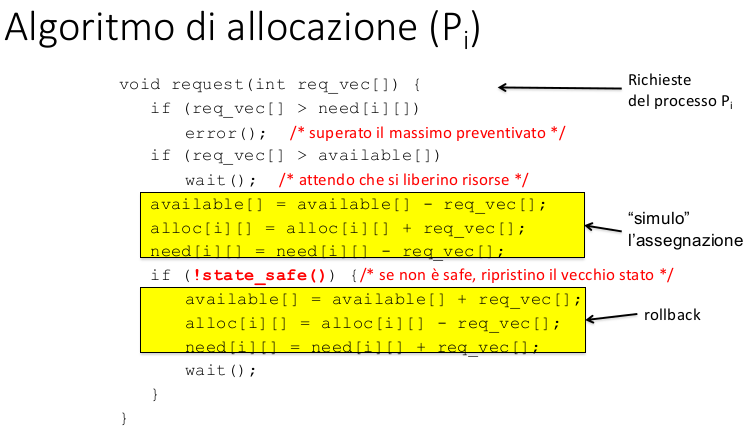
\includegraphics[width=1\textwidth]{banchiere1.png}
\end{center}

\begin{center}
    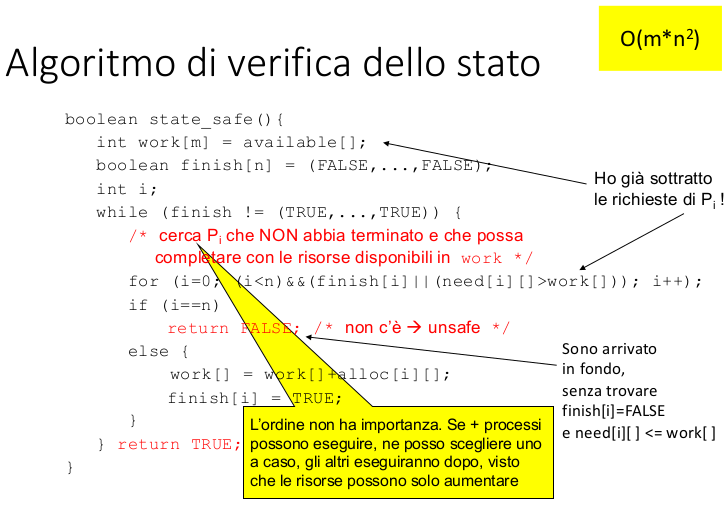
\includegraphics[width=1\textwidth]{banchiere2.png}
\end{center}
3) L'algoritmo di rilevazione permette che ci siano dei Deadlock, ogni tanto verifica che il sistema sia caduto in Deadlock
 in un metodo simile all'algoritmo del banchiere senza la necessità di conoscere la matrice max, verifica solo se il sistema è in 
 uno stato SAFE. Usa strutture dati simili a quello del banchiere.
 \begin{center}
     \begin{verbatim}
         int available[m]; //n° istanze di R_i disponibili
         int alloc[n][m]; //matrice allocazione corrente
         int req_vec[n][m]; //matrice di richiesta,
                            //stesse dimensione della max,
                            // è una max istantanea
     \end{verbatim}
 \end{center}
 \begin{center}
     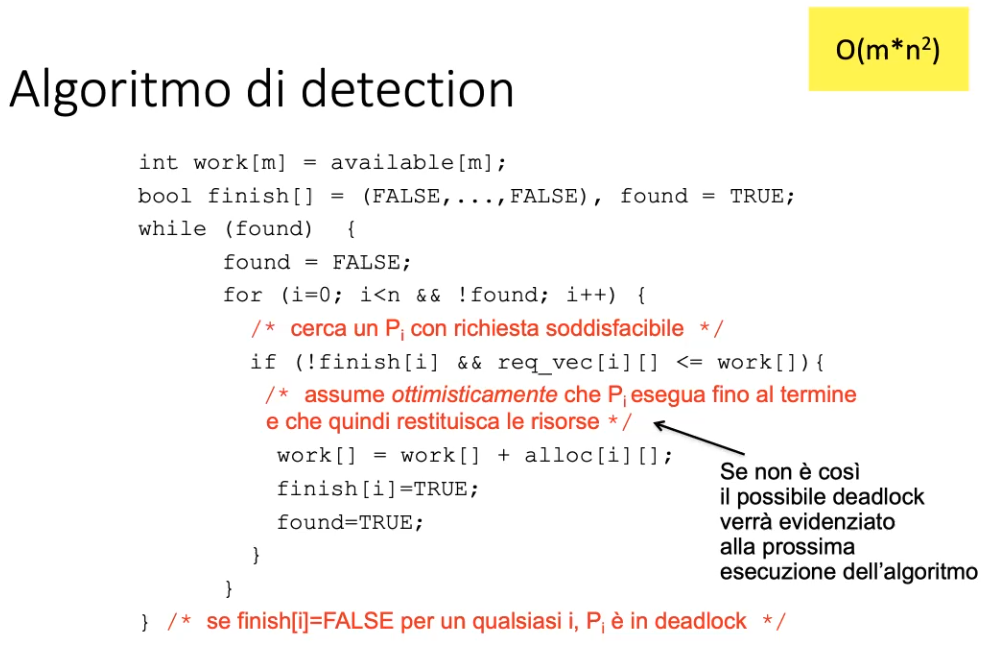
\includegraphics[width=1\textwidth]{detection.png}
 \end{center}
 Parte dal presupposto che tutti i processi siano bloccati,
 verifica se il singolo processo non ha finito e se le risorse che richiede siano inferiori a quelle disponibili.
  come trova un processo che può proseguire
  con la sua esecuzione significa che non si è in Deadlock, non verifica la situazione futura, solo quella attuale.
Esempio:
\begin{center}
    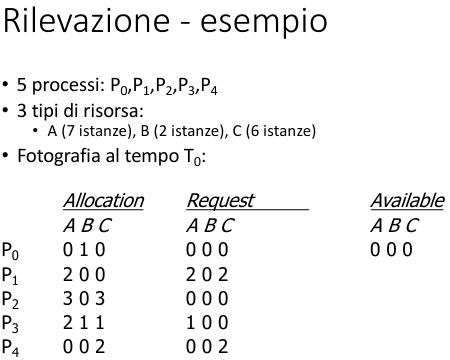
\includegraphics[width=1\textwidth]{detection2.png}
\end{center}
Usando l'algoritmo si passa man mano ogni singolo processo e si verifica se nello stato attuale può finire la sua esecuzione
 oppure è fermo a causa di un'attesa di risorse. Man mano che si trovano processi che possono concludere, si considerano 
 le risorse in loro possesso come possibili risorse future disponibili.

 L'algoritmo di rilevazione può essere lanciato:
 \begin{itemize}
     \item dopo ogni richiesta di risorsa
     \item ogni N secondi
     \item quando la percentuale di utilizzo della CPU cala sotto una soglia T
 \end{itemize}
 La prima è particolarmente costosa, non si fa prevenzione, ma si verifica sempre, che può essere problematico essendo 
 un algoritmo che può arrivare ad avere una complessità cubica. La terza opzione potrebbe non rilevare dei Deadlock causati da 
 piccoli gruppi di processi che non causano grossi cali d'uso della CPU.

 Quando ci si accorgerà del Deadlock si potrà:
 \begin{itemize}
     \item uccidere tutti o alcuni dei processi coinvolti
     \item prelazionare tutti i processi coinvolti
 \end{itemize}
 In entrambi i casi sarebbe un grosso danno, perché i processi hanno lavorato fino a quel momento  
 per niente.
 Per la prima, invece di uccidere tutti i processi si può scegliere di ucciderne uno alla volta in base a 
 alle risorse allocate, a quante ne mancano, a quanto tempo mancava, etc e verificare dopo se il Deadlock 
 è tuttora presente o meno.
 La seconda possibilità invece porta il problema che prelazione un singolo processo equivale quasi a ucciderlo 
 visto che non può continuare normalmente come prima, una possibile soluzione è il \textbf{rollback} che comporta
 un lavoro in precedenza eseguito dalla CPU per salvare uno stato in cui il processo non era bloccato.
 Successivamente quest potrebbe causare un fenomeno di starvation se si andrà a fare \textbf{rollback} dei soliti
 processi, in quel caso una possibile soluzione potrebbe essere quella di considerare il numero di \textbf{rollback}
 nei fattori di costo.

 \section{Gestione della memoria}

 Un processo ha bisogno sia di memoria RAM che di memoria di massa per poter lavorare. La memoria serve ai processi per
 via dell'uso del \textbf{Program Counter} da parte della CPU .
 Possono nascere svariati problemi nella gestione della memoria per i processi:
 \begin{itemize}
     \item l'allocazione della memoria dei singoli processi
     \item protezione dello spazio allocato
     \item condivisione dello spazio allocato
     \item gestione dello swap
     \item gestione della memoria virtuale
 \end{itemize}
 Ogni programma per essere eseguito deve essere messo in memoria e trasformato in processo, da quel momento la CPU
 preleverà istruzioni dalla memoria in base al \textbf{Program Counter}, questo può portare all'ulteriore prelievo di dati dalla
 memoria fino alla fine dell'esecuzione con l'eventuale scrittura in memoria del risultato, una volta che il processo terminerà
 la memoria verrà rilasciata.

 \paragraph{Come avviene il passaggio da programma a processo?}
 La trasformazione avviene tramite una trasformazione di indirizzi di memoria.
 \begin{center}
     \begin{verbatim}
         int x = 3;
     \end{verbatim}
 \end{center}
 non è altro che un riferimento a un indirizzo di memoria, quando il programma verrà eseguito, quell'indirizzo
 \textbf{simbolico} verrà tradotto in un indirizzo \textbf{fisico}.
 \paragraph{Chi compie questa trasformazione?}
 \begin{description}
     \item [il compilatore:] prende l'indirizzo \textbf{simbolico} e lo trasforma in una serie di indirizzi \textbf{rilocabili}
     ovvero che si possono posizionare da un'altra parte
     \item [il linker e/o il loader:] prendono l'indirizzo \textbf{rilocabile} e lo trasformano in indirizzo fisico assoluto
 \end{description}
 Possono essere coinvolti tutti o no, in base a come avviene la trasformazione.
 \begin{center}
     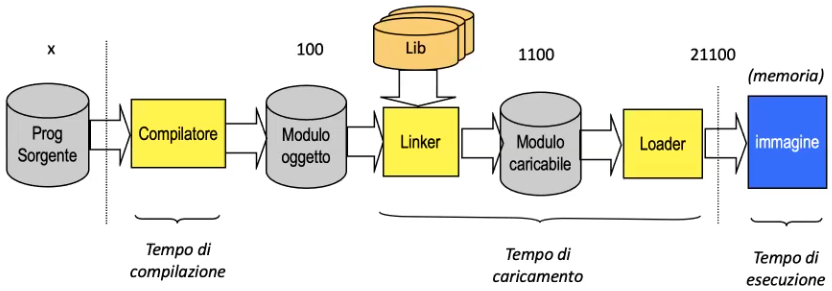
\includegraphics[width=1\textwidth]{trasformazione.png}
 \end{center}
La variabile X viene presa dal \textbf{compilatore} e trasformata da indirizzo \textbf{simbolico} a indirizzo \textbf{rilocabile}, viene
creato un modulo oggetto, in cui alla variabile viene assegnato un indirizzo di memoria, X non sarà più X, sarà l'area di memoria
all'indirizzo 100. Il \textbf{linker} collegherà l'indirizzo 100 con gli indirizzi delle eventuali librerie incluse nel programma,
ciò causerà la creazione di un modulo ricaribile in memoria. La X dall'indirizzo 100 sarà spostata all'indirizzo 1100 per fare spazio
alle eventuali librerie. Il modulo caricabile è quello che effettivamente verrà caricato in memoria dal \textbf{loader}. Il SO
assegnerà uno spazio all'interno della memoria tenendo conto dello spazio effettivamente occupato al momento. Eventualmente se
l'indirizzo 1100 fosse occupato, il SO potrà spostarlo a un altro indirizzo libero, fatto questo il processo verrà eseguito.
Se si troverà un'istruzione 
\begin{center}
    \begin{verbatim}
        int a = x + b;
    \end{verbatim}
\end{center}
vedendo che l'operando da prelevare è X, verrà ripescato dall'indirizzo di memoria, tale azione che collega indirizzi 
\textbf{simbolici} a indirizzi \textbf{fisici} viene denominata \textbf{binding degli indirizzi}.
\subsection{Tempi di compilazione}
\begin{description}
    \item[compile-time:] avviene a tempo di compilazione,in quel caso ci sarà solo il 
    \textbf{compilatore} che non può sapere se l'indirizzo che assegna al programma sia occupato o meno, di conseguenza 
    in caso in cui fosse occupato il programma semplicemente non verrà eseguito. Ciò funziona bene se la memoria è ottimizzata
    al massimo. Per cambiare la locazione del programma l'unica opzione sarà quellla di ricompilarlo.
    \item[load-time:]avviene a tempo di caricamento, il \textbf{loader} può notare che l'area di memoria in cui vuole
    caricare sia occupata e di conseguenza cambia l'area in cui andare a caricare. Il codice sarà rilocabile, anche se non permette
    di spostare il processo mentre è in esecuzione. Se cambiasse l'indirizzo di riferimento sarà necessario ricaricare.
    \item[run-time:]permette di spostare l'indirizzo di memoria allocato mentre il processo è in esecuzione, è necessario un 
    supporto hardware perché decisamente più efficiente. 
\end{description}
I primi due tipi di \textbf{binding} sono considerati \textbf{statici} mentre l'ultimo è considerato \textbf{dinamico}.

\subsection{Linking}

Può essere diverso indipendentemente dal tipo di \textbf{binding}.
\begin{description}
    \item[statico:] tradizionale, prima di mandare in esecuzione il processo, si è creato un'immagine di memoria con 
    tutte le librerie incluse.
    \item[dinamico:]il sistema viene preparato per accogliere un'immagine del codice e delle librerie, ma il linking vero e
    e proprio avverrà solo al momento dell'esecuzione, l'eseguibile sarà più piccolo perché non conterrà le librerie, ma solo 
    il loro riferimento.  
\end{description}

Un programma linkato staticamente occuperà una maggior memoria rispetto a un programma linkato dinamicamente, dal punto di vista
di caricamento il dinamico vince sullo statico, in quel caso gli stub creati dal linkato dinamico dovranno essere completati a 
\textbf{run-time} e ciò porterà il programma a essere più lento rispetto a quello linkato staticamente.

Ricapitolando:
\begin{description}
    \item[linking statico:]\begin{itemize}
        \item occupa maggior memoria
        \item lento nel caricamento
        \item veloce nell'esecuzione
    \end{itemize} 
    \item[linking dinamico:]\begin{itemize}
        \item occupa meno memoria
        \item più rapido nell'avvio
        \item più lento nell'esecuzione
    \end{itemize}
\end{description}

\subsection{Loading}

Lo stesso concetto di statico e dinamico può essere applicato al \textbf{loader}.
\begin{description}
    \item[statico:] tutto il codice viene caricato in memoria al tempo di esecuzione, quindi deve essere disponibile in 
    memoria prima di eseguire il programma
    \item[dinamico:] i moduli che servono al processo vengono caricati al primo utilizzo, se una parte non serve non verrà
    caricata di conseguenza 
\end{description}

Uno dei malus dello \textbf{statico} è la possibilità di programmi in cui una parte del codice non verrà mai eseguita (magari
per via di condizioni), non conviene di conseguenza caricare completamente il programma, in quel caso il loading \textbf{dinamico}
diventa decisamente più utile.

\subsection{Spazio di indirizzamento logico}

Consiste nello spazio visto dalla CPU quando esegue un processo, mappato su uno spazio di indirizzamento fisico in RAM. Il SO 
deve mappare indirizzi logici o virtuali su indirizzi fisici reali, quando si fa \textbf{binding} a \textbf{compile-time} o
\textbf{load-time} l'indirizzo logico e fisico coincidono. Invece con un \textbf{binding} a \textbf{run-time} l'indirrizzo
logico generato dalla CPU potrebbe non coincidere con quello fisico presente in RAM, tutto ciò viene sempre gestito dal
SO. Una gestione dinamica come questa ha un costo, ovvero il tempo che ci mette la MMU (Memory Management Unit) che tiene 
conto del riferimento tra indirizzo logico a quello fisico a tradurre la richiesta.

La MMU può essere composta da un registro e un sommatore che somma gli indirizzi logici con un offset, potrebbe essere problematico
con processi che dovrebbero essere divisi all'interno dello spazio di memoria.

\section{Schemi di gestione della memoria}

\subsection{Allocazione contigua}

L'immagine di memoria del processo sarà tutto allocato in un'area contigua per l'appunto, senza buchi in mezzo. Per gestire
l'allocazione in questo modo esistono delle varianti:

\subsubsection{Partizioni fisse}

La memoria è divisa a blocchi, ciascun blocco con una determinata
    dimensione che rimarrà fissa per sempre, tra di loro possono essere variabili, ma rimangono fisse. Il processo che arriva
    verrà posizionato nella prima partizione che permette di contenerlo. Un contro è che se un blocco viene occupato solo in 
    parte, quella libera sarà sprecata, perché il blocco è fisso e non può essere partizionato. Esistono delle opzioni:

    \begin{itemize}
        \item un'unica coda di attesa, con i processi in fila e come si libera uno spazio il processo in testa verificherà
        se riesce a entrarci o meno
        \item tante code, una per partizione, il SO fa un preselezione del processo che verrà messo nella coda più adatta a lui
    \end{itemize}

    Entrambe hanno vantaggi e svantaggi, una coda per partizione causerà la possibilità di avere delle code vuote e altre piene 
    in quel caso si avrebbe tanta memoria sprecata e pochi processi in coda. Va bene solo nel caso in cui il carico dei vari processi
    è ben distribuito e di varie dimensioni. Se tutte le code fossero piene, sarebbe ottimale per l'uso della memoria.

    Nell'alternativa con un'unica coda, la gestione sarà più complicata, perché un processo troppo grande per stare in partizioni
    troppo piccole rimarrebbe in attesa in caso di algoritmo FCFS, bloccando tutti gli altri processi dietro di lui che 
    potrebbero entrare nelle partizioni libere. Una scansione della coda quando si libera una partizione risolve il problema, ci 
    sono due varianti
    
    \begin{description}
        \item[best-fit:] scansiona tutta la coda scegliendo quello più adatto alla partizione che si è liberata
        ovvero quello che si avvicina a occuparla maggiormente, se la coda è molto lunga il tempo impiegato sarà decisamente
        elevato
        \item[best-available-fit:] viene scelto il primo processo che può stare nella partizione che si è liberata, non minimizza
        lo spreco, perché potrebbe esserci un processo che occuperebbe meglio la partizione 
    \end{description}

Lo schema della MMU con un allocazione contigua a partizioni fisse è il seguente:

\begin{center}
    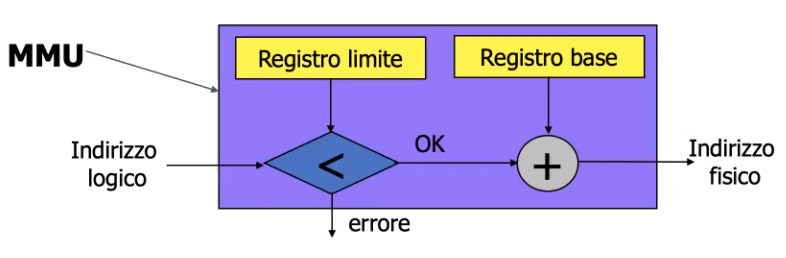
\includegraphics[width=1\textwidth]{mmu_partizioni_fisse.png}
\end{center}

Pro e contro:

\begin{description}
    \item[pro:] semplicità, il SO deve solo tenere traccia di una tabella in cui si definisce in quale partizione andrà il processo
    \item[contro:] il livello di multiprogrammazione è vincolato dal numero di partizioni, inoltre c'è uno spreco di memoria causato
    dalla frammentazione della memoria:
    
    \begin{description}
        \item[interna:] causata dall'assegnamento di un processo a una partizione che non viene occupata al 100%
        \item[esterna:] la somma della parte libera di partizioni parzialmente occupate potrebbe essere grande a sufficienza
        per un processo che invece sarà costretto ad attendere 
    \end{description}
    la frammentazione riduce l'efficacia nell'uso della memoria, la tecnica con partizioni fisse soffre di entrambe, è più adatta per
    processi delle dimensioni giuste ed esatte alle partizioni che si vogliono occupare, quindi più verso i sistemi embedded.
\end{description}

\subsubsection{Partizioni variabili}

Il processo che arriva in memoria si prenderà una fetta di memoria grande esattamente quanto lo spazio che occuperebbe.
La frammentazione esterne rimarrà, esempio:

\begin{itemize}
    \item si crea una partizione da 100, una da 50, una da 30 e una da 20
    \item si libera quella da 50 e da 20
    \item un processo che occupa 70 potrebbe entrare se le posizioni da 50 e 20 venissero sommate, ma non si può a causa dell'allocazione contigua
\end{itemize}

L'effetto a "groviera" che si genera 
 
\end{document}